\documentclass[12pt,a4paper]{article}
\usepackage{amsmath}
\usepackage[english]{babel}
\usepackage{graphicx}
\usepackage{listings}
\usepackage{fullpage}
\usepackage[T1]{fontenc}

\lstdefinestyle{custompython}{
  belowcaptionskip=1\baselineskip,
  breaklines=true,
  frame=L,
  xleftmargin=\parindent,
  language=bash,
  basicstyle=\footnotesize\ttfamily,
  showstringspaces=false,
  %commentstyle=\itshape\color{purple!40!black},
  %keywordstyle=\itshape\color{green!40!black},
  %identifierstyle=\color{blue},
  %stringstyle=\color{orange},
}

\author{
  Cheng, Lidens\\
  \texttt{lidenscheng@email.arizona.edu}
  \and
  McClintock, Tom\\
  \texttt{tmcclintock@email.arizona.edu}
  \and
  Wagoner, Erika\\
  \texttt{wagoner47@email.arizona.edu}
}
\title{Astr 513: Homework 1}

\begin{document}
\maketitle
  
\section{Random Number Generators}
Our pseudo-random number generator (PRNG) of choice is the Mersenne Twister, MT19937. It was developed by Makoto Matsumoto and Takuji Nishimura in 1997. The algorithm generates a sequence of word vectors of size $w$, which are uniform pseudo-random integers in $[0,2^w-1]$. After dividing by $2^w-1$, the word vectors become real numbers in $[0,1]$. The linear recurrence relation for each word is a twisted version of a generalized feedback shift register, which consists of bitwise shifts, ORs, XORs, and matrix multiplication [1][2]. \\\\ 
Parameters have been chosen so that MT19937 has a long period of $2^{19937}-1$. The output is equidistributed in $k=623$ dimensions for 32-bit words. This means it would only exhibit patterns when $k \geq 623$ dimensions [1][2]. Thus, clustering does not seem to be a big issue with MT19937.\\\\
MT19937 is not particularly space efficient. The generator state takes up 2500 bytes of RAM ($625 \times 32$ bits) [3]. It passes most of the statistical randomness tests, but not all of the most stringent ones. This is most applicable to instances where two seeds are extremely similar. In such a case, MT19937 can take a long time before the two sequences of numbers would diverge. This issue has been addressed in an update [4]. In terms of speed, MT19937 has been evaluated to generate approximately $138.889$ million random numbers per second, $7.2$ns for each number, and at $44\%$ of the speed relative to the fastest PRNG [5]. \\\\
Although it might not be the most efficient PRNG, MT19937 is extremely portable. It comes default in numerous general purpose, programming languages and softwares such as C++, Python, R, MATLAB, and IDL. In addition, it is available in a 64-bit variety. MT19937 is a reliable PRNG independent of the compiler or system being used.  

\section{Designing surveys}
We are given a prior probability from the rate of detecting planets of $1-2 R_{\oplus}$ around solar type stars from Kepler, and are told to assume this rate has been measured to high accuracy as being 10\%. We are tasked with determining the number of solar type stars we would need to observe to find at least 30 $1-2 R_{\oplus}$ planets in a similar survey observing a different area of the sky with a 90\% and 99\% likelihood. To do this, we will want to make use of the binomial distribution,
\begin{equation*}
  P(n, \rho | N) = \left(N \choose n\right) \rho^n \left(1 - \rho\right)^{N - n},
\end{equation*}
where $n$ is the number of successes, $\rho$ is the prior likelihood of obtaining a success, and $N$ is the number of independent observations. We will want to solve for $N$ given a probability of 0.9 or 0.99, but there is a modification that needs to be made because we want the probability not of finding exactly 30 of theses planets, but 30 or more of them. There are two ways to calculate this probability, either by adding the probabilities of finding $n \in {[30, \infty]}$ planets, or by adding the probabilities of finding $n \in {[0, 29)}$ planets and subtracting this sum from 1. Computationally, the latter of these is the most logical, so our probability will actually be
  \begin{equation*}
    P(n \ge 30, \rho | N) = \sum_{m = 0}^{29} \left(N \choose m\right) \rho^m \left(1 - \rho\right)^{N - m},
  \end{equation*}
  and when solving we will use the substitution that $\rho = 0.1$ and $P(n \ge 30, \rho | N) = 0.9$ or $0.99$.\\\\
Using a false position method root finding algorithm in Python, we were able to find the values of $N$ that would satisfy the above equation for our desired likelihoods. These values are
\begin{description}
  \item [\normalfont a)]$N = 368$ for a 90\% likelihood
  \item [\normalfont b)]$N = 435$ for a 99\% likelihood
\end{description}

\section{Blackbody Distribution}
\subsection{}
Given our initial distribution:
\begin{equation*}
  f(\epsilon;T)d\epsilon = C\frac{\epsilon^2d\epsilon}{\exp{(\epsilon/kT)}-1}
\end{equation*}
we first make a change in variables $\epsilon' = \epsilon/kT$. This results
in the distribution
\begin{equation*}
  f(\epsilon')d\epsilon' = A\frac{\epsilon'^2d\epsilon'}{\exp{(\epsilon')}-1}
\end{equation*}
where $A=C(kT)^2$.
\subsection{}
We now need to find where this function is a maximum numerically. First we
define our function in Python:
\begin{lstlisting}[style=custompython]
  def f(eps):
      return eps**2/(np.exp(eps)-1)
\end{lstlisting}
and find its maximum. This was found to be at the 
location $\epsilon'\approx1.594$.
\subsection{}
We now renormalize by dividing by $f(\epsilon=1.594)\approx0.6476$.
This yields:
\begin{equation*}
  f'(\epsilon')d\epsilon' = B\frac{\epsilon'^2d\epsilon'}{\exp{(\epsilon')}-1}
\end{equation*}
where $B=A/0.6476$.
\subsection{}
We define a function to return a photon of energy between $\epsilon'_1=0.1$
and $\epsilon'_2=5.0$.
\begin{lstlisting}[style=custompython]
  def en(eps):
      return np.random.rand()*(5.0-0.1)+0.1
\end{lstlisting}
\subsection{}
We now make repeated draws to this function to get a collection of $N$
photon energies ${e_i},\ i\in[1,N]$. Additionally, we draw $N$ random
numbers between $0$ and $1$, ${r_i},\ i\in[1,N]$. If $f'(\epsilon'_i) < r_i$
then the photon is removed from the list. We do this for $N=100000$.
\subsection{}
Histogramming the photons yields a version of the distribution
with the area of the bins normalized to $1$.
\begin{figure*}[!h]
  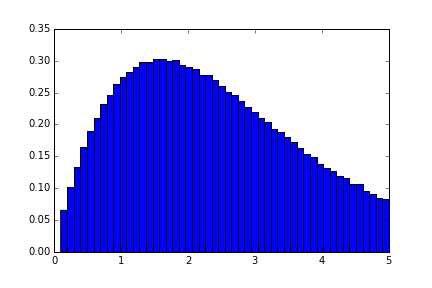
\includegraphics[]{HW1_3_6_normalized.png}
\end{figure*}
\newpage
\noindent
If we simply loop over the energy domain and plot the fraction of accepted
photons in that bin then we recover $f'$.
\begin{figure*}[!h]
  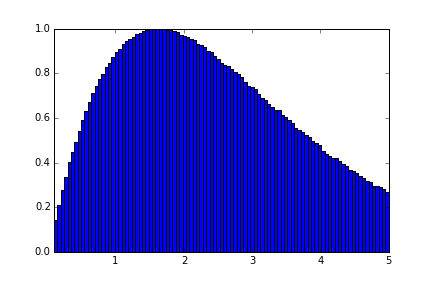
\includegraphics[]{HW1_3_6.png}
\end{figure*}

\newpage

\section*{References}

\begin{enumerate}
  \item Matsumoto, Makoto, and Takuji Nishimura. "Mersenne Twister: A 623-dimensionally Equidistributed Uniform Pseudo-random Number Generator." Transactions on Modeling and Computer Simulation. TOMACS ACM Transactions on Modeling and Computer Simulation 8.1 (1998): 3-30.
  \item Tian, Xiang, and Khaled Benkrid. "Mersenne Twister Random Number Generation on FPGA, CPU and GPU." 2009 NASA/ESA Conference on Adaptive Hardware and Systems (2009): Web.
  \item Matsumoto, Makoto. "Mersenne Twister with Improved Initialization." Hiroshima University. Web. http://www.math.sci.hiroshima-u.ac.jp/~m-mat/MT/MT2002/emt19937ar.html.
  \item "Pseudo-Random Number Generator." Boost C++ Libraries. Web. \\ http://www.boost.org/doc/libs/1{\_}46{\_}1/doc/html/boost{\_}random/reference.html.
  \item "Performance." Boost C++ Libraries. Web. \\ http://www.boost.org/doc/libs/1{\_}46{\_}0/doc/html/boost{\_}random/performance.html.   
\end{enumerate}

\end{document}
